\begin{surferPage}[216 Синг.]{Поверхности со множеством действительных сингулярностей.}
    Как говорилось выше, уже для поверхностей седьмого порядка неизвестно, каково максимальное количество $\mu(7)$ точек сингулярности на них, известно лишь, что справедливо условие: $99\le \mu(7) \le 104$. 

Поэтому не удивительно, что для произвольного порядка d сведений ещё меньше. Соня Бреске, Оливер Лабс и Дуко ван Стратен смогли по меньшей мере изменить конструкцию С.В. Чмутова так, что известный на сегодняшний день максимум количества сингулярностей $\mu(d)$ достигается и действительными сингулярностями. Поэтому известно следующее: 
    \[0,41\bar{6}d^3 \lessapprox \mu(d) \lessapprox 0.44\bar{4} d^3.\]
Глядя сверху, можно увидеть симметрию конструкции и её взаимосвязь с вопросом о максимальном количестве черных клеток в изображенной конфигурации прямых:
    \begin{center}
      \begin{tabular}{c@{\qquad}c}
        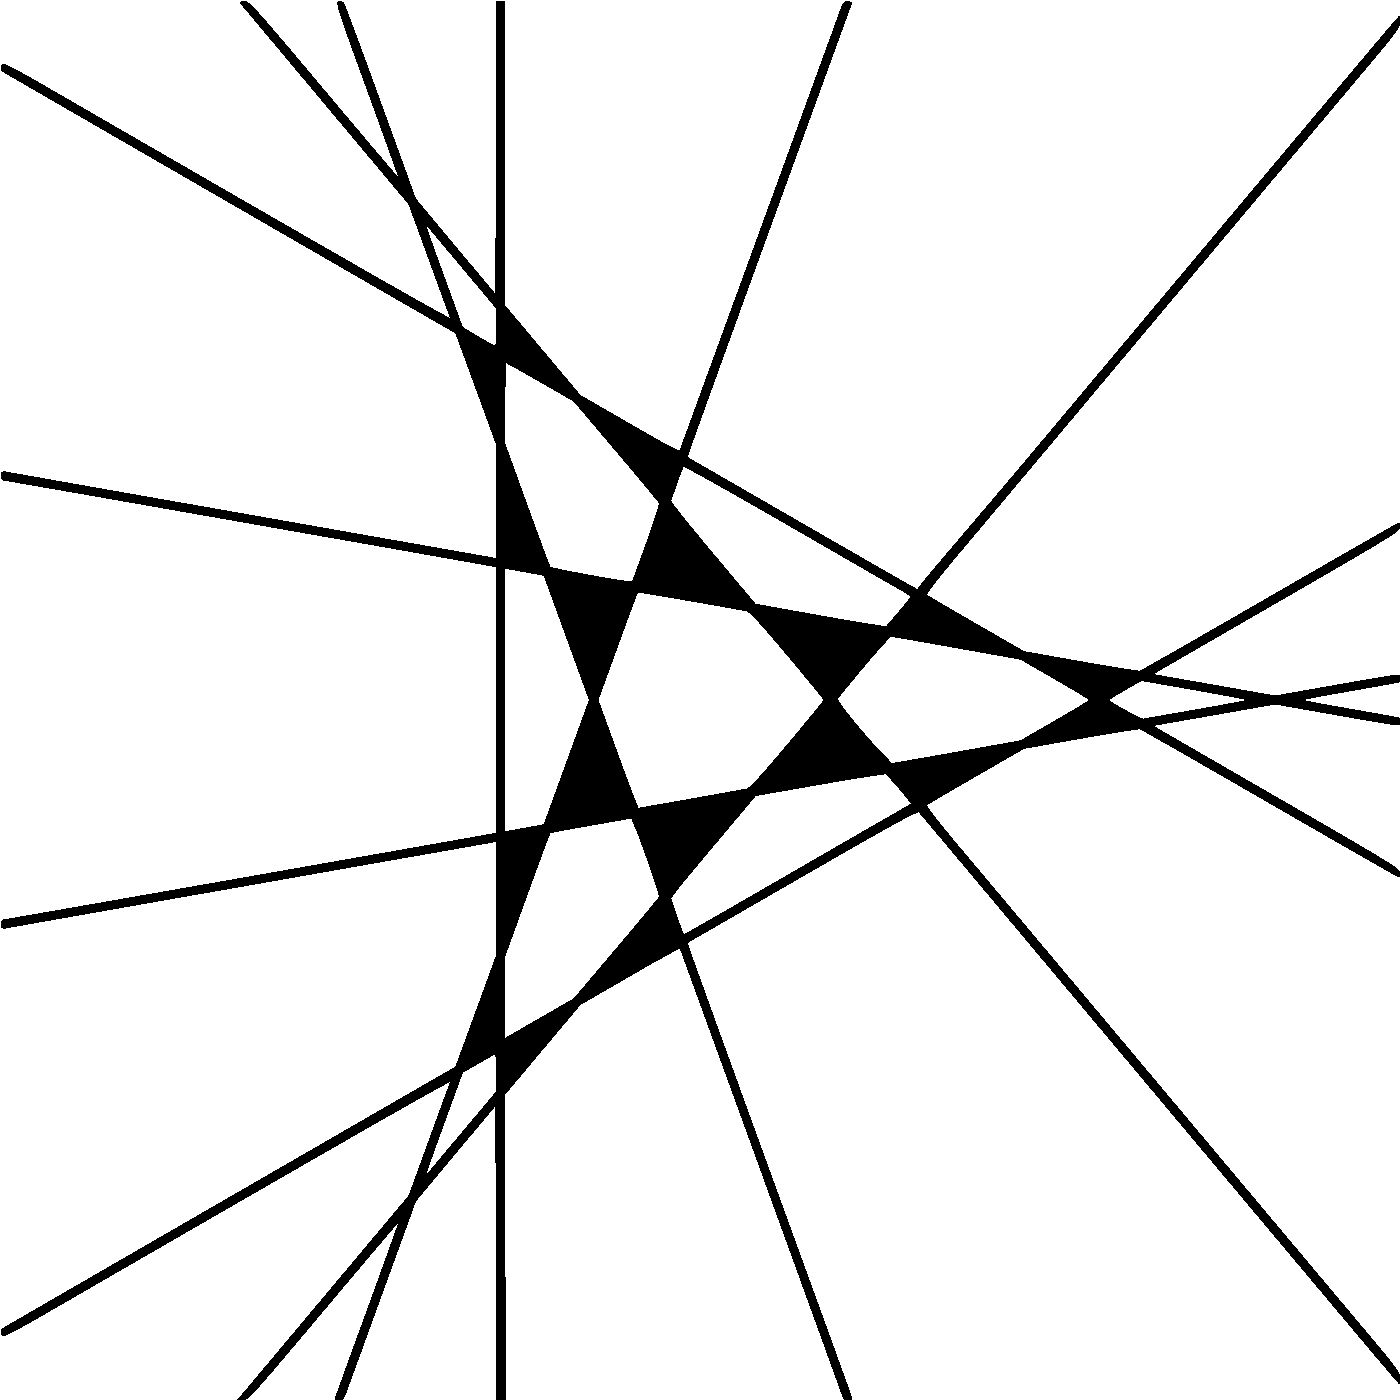
\includegraphics[height=1.5cm]{vielesing.pdf}
        &
        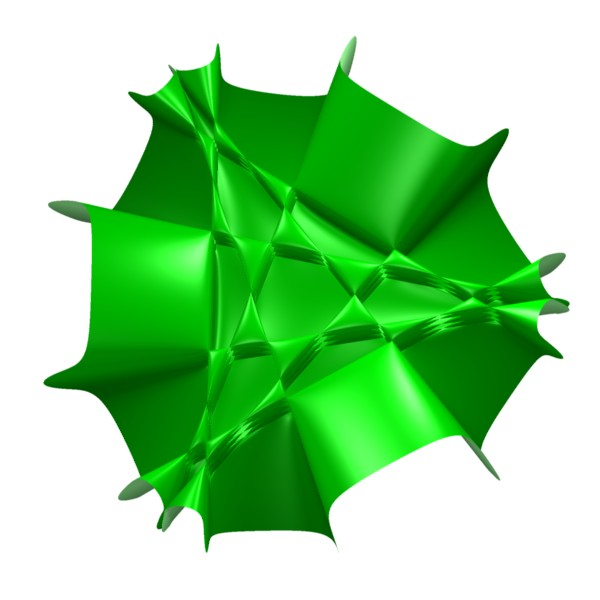
\includegraphics[height=1.5cm]{p9surface_von_oben}
      \end{tabular}
    \end{center}
\end{surferPage}
